\documentclass{beamer}

\mode<presentation> 
{
    \usetheme{Madrid}
}

\usepackage[utf8x]{inputenc}
\usepackage[english,russian]{babel}
\usepackage[T2A]{fontenc}
\usepackage{graphicx}
\usepackage{booktabs} 
\usepackage{mathtools}
\usepackage{amsmath}
\usepackage{wasysym}
\usepackage{subfig}
\usepackage{hyperref}
\usepackage{ulem}
\usepackage{ragged2e}
\usepackage{algorithm2e}
\usepackage{minted}

\usemintedstyle{borland}

\usefonttheme[onlymath]{serif}

\hypersetup
{
    colorlinks=true,
    linkcolor=white, 
    urlcolor=cyan
}

\title[Лекция 1]
{
    Лекция 1: Цифровая фильтрация (продолжение) и типы в языке программирование Си 
} 


\author[Д. А. Караваев]{Д. А. Караваев}

\institute[СПбГУТ] 
{
    Санкт-Петербургский государственный университет телекоммуникаций \\ им. проф. М. А. Бонч-Бруевича \\ 
    \vspace{0.2cm}
    Факультет РТС, Кафедра РОС \\
    \vspace{0.2cm}
    Факультатив <<Программирование в ЦОС>> \\
    \vspace{0.2cm}
    Осень 2019
}

\date[14.10.2019]{14.10.2019 Санкт-Петербург} 

\begin{document}
    \begin{frame}
        \titlepage 
    \end{frame}
    \begin{frame}
        \frametitle{Комплексные числа}
        \justifying
        В радиотехнических приложениях ЦОС повсеместно используется комплексное $\textrm{IQ}$ представление сигнала: 
        \begin{equation}
            \textrm{U}[n] = \textrm{I}[n] + j \textrm{Q}[n] = a[n] \cos(\varphi[n]) + a[n] j\sin(\varphi[n]), \label{eq:IQ}
        \end{equation}
        где $a[n],\ \varphi[n]$ - изменение амплитуды и фазы сигнала, а $\textrm{U}[n]$ - {\it комплексная огибающая} (дискретизированная) несущего колебания.
        \par
        Будем рассматривать произвольные комплексные сигналы (необязательно имеющие $\textrm{IQ}$ интерпретацию):
        \begin{equation}
            s[n] = \textrm{Re}\{s[n]\} + j\textrm{Im}\{s[n]\},\ s[n] \in \mathbb{C}. \label{eq:complex}
        \end{equation}
    \end{frame}
    \begin{frame}
        \frametitle{DDC}
        \justifying
        Одним из первичных этапов цифровой обработки радиосигналов является перенос {\it вещественного} сигнала с АЦП с {\bf промежуточной частоты} (ПЧ) на 0 (получение {\it комплексной огибающей}) и установление необходимой $F_{s}$ путём децимации: 
        \begin{figure}[!tbp]
           \centering
           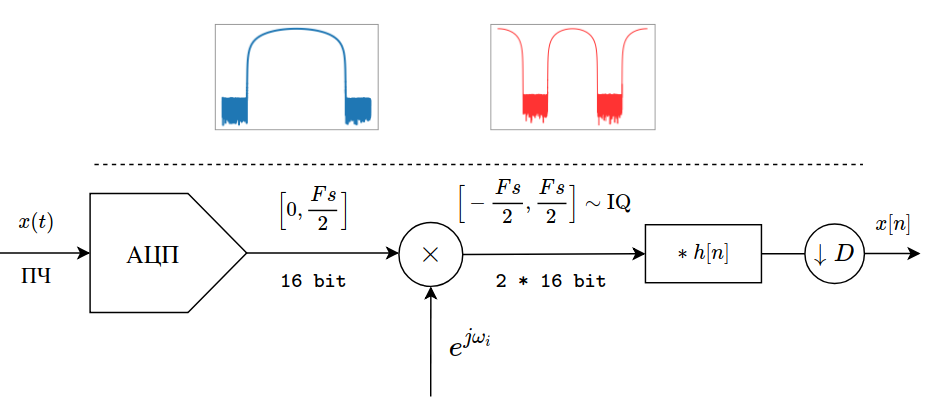
\includegraphics[width=0.85\textwidth]{pics/DDC.png}
           \captionsetup{justification=centering}
           \captionof{figure}{Схема Digital Down Converter}
       \end{figure}
    \end{frame}
    \begin{frame}
        \frametitle{КИХ-фильтр для комплексных сигналов}
        \justifying
        Пусть входной сигнал КИХ-фильтра $x[n]$ является комплексным, а ИХ по-прежнему вещественная $h[n]$ длины $T$, тогда:
        \begin{equation}
        \begin{split}
            y[n] &= x[n] * h[n] = \sum_{k = 0}^{T-1}h[k]x[n - k] = \\
                 &= \sum_{k = 0}^{T-1}h[k]\textrm{Re}\{x[n - k]\} + j\sum_{k = 0}^{T-1}h[k]\textrm{Im}\{x[n - k]\} = \\
                 &= \textrm{Re}\{x[n]\} * h[n] + j\textrm{Im}\{x[n]\} * h[n], \label{eq:cconv}
        \end{split}
        \end{equation}
        \par
        {\bf Вывод:} Комплексная фильтрация $\implies$ фильтрация вещественной и мнимой части по отдельности.
        \par
    \end{frame}
    \begin{frame}{Псевдокод алгоритма комплексной свёртки}
        \begin{algorithm}[H]
            \SetKwInOut{Input}{Вход}
            \SetKwInOut{Output}{Выход}
            \Input{$\hat x[n] \in \mathbb{C}$ - вх. сигнал длины $N + T - 1$, $h[n] \in \mathbb{R}$ - ИХ длины $T$.}
            \Output{$y[n] \in \mathbb{C}$ - вых. сигнал длины $N$.}
            \BlankLine
            \For{$n \leftarrow 0$ \KwTo $N - 1$} 
            {
                $\textrm{Re}\{y[n]\} \leftarrow 0$
                \par
                $\textrm{Im}\{y[n]\} \leftarrow 0$
                \par
                $m \leftarrow n + (T - 1)$
                \par
                \For{$k\leftarrow 0$ \KwTo $T - 1$}
                {
                    $\textrm{Re}\{y[n]\}  \leftarrow \textrm{Re}\{y[n]\} + \textrm{Re}\{\hat x[m - k]\} h[k]$
                    \par
                    $\textrm{Im}\{y[n]\}  \leftarrow \textrm{Im}\{y[n]\} + \textrm{Im}\{\hat x[m - k]\} h[k]$
                }
            }
        \end{algorithm}
        {\bf Замечание:} Необходимо разобраться, как в языке программирования Си можно представить комплексные числа.
    \end{frame}
    \begin{frame}[fragile]
        \frametitle{Фильтрация без усиления}
        \justifying
        В приложениях часто требуется, чтобы амплитуда в полосе пропускания фильтра вых. сигнала $y[n]$ {\it значительно} не изменялась по сравнению с вх. сигналом $x[n]$:
        \begin{equation}
        \begin{split}
            h[n] &\leftarrow \frac{h[n]}{|H(e^{j\omega_{0}})|},\ \omega_{0} = 0, \implies \Biggl\lvert \sum_{k=0}^{T-1} h[k] \Biggr\lvert = 1, \\
            H(e^{j\omega}) &= \sum_{k=0}^{T-1} h[k]e^{j\omega k},\\
            |H(e^{j\omega_{0}})| &= \Biggl\lvert \sum_{k=0}^{T-1} h[k]e^{j\omega_{0} k} \Biggr\lvert = \Biggl\lvert \sum_{k=0}^{T-1} h[k] \Biggr\lvert \\
        \end{split}
        \end{equation}
        \par
        {\bf Вопрос:} Что делать с условием $(4)$ для целых чисел (типа ${\tt int}$)? 
    \end{frame}
    \begin{frame}
        \frametitle{Приведение ИХ}
        {\bf Решение:} $$h_{\texttt{int}}[n] = \big\lfloor \texttt{int}_{\textrm{max}} \times  h_{\texttt{float}}[n] \big\rfloor \implies y_{\texttt{int}}[n] = \frac{1}{\texttt{int}_{\textrm{max}}}(x_{\texttt{int}}[n] * h_{\texttt{int}}[n]).$$
        \begin{figure}[!tbp]
           \centering
           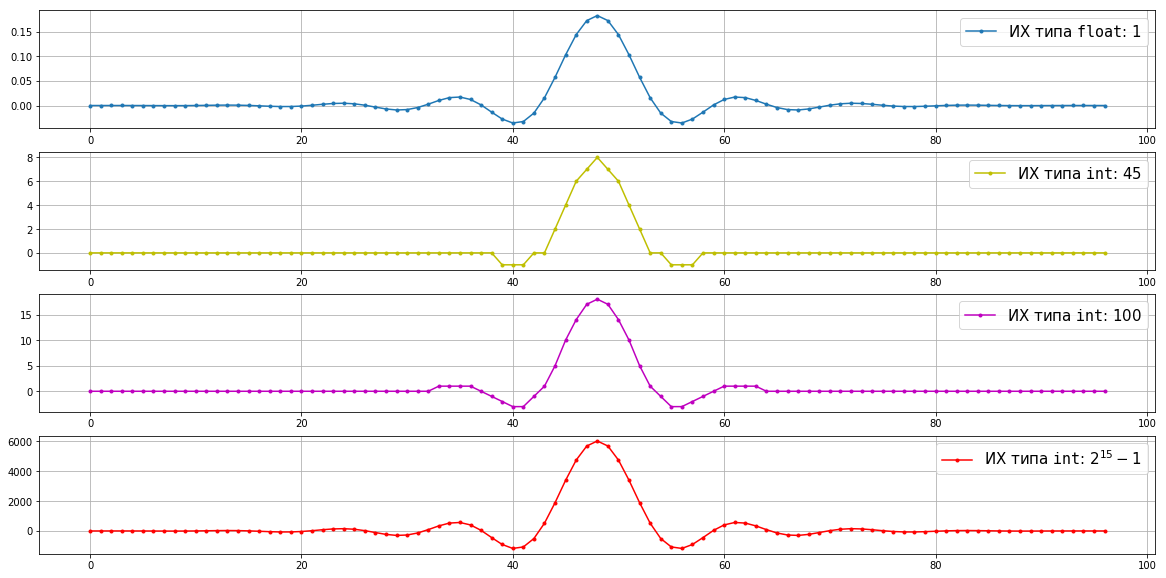
\includegraphics[width=0.88\textwidth]{pics/IR.png}
           \captionsetup{justification=centering}
           \captionof{figure}{Динамика значений ИХ}
       \end{figure}
    \end{frame}
    \begin{frame}[fragile]{Представление комплексных чисел в языке Си}
        \begin{minted}[frame=lines,        framesep=2mm,
                       baselinestretch=1.2, fontsize=\footnotesize,
                      linenos]{c}
/* В языке Си есть встроенные конструкции для комплексных чисел,
 * но мы их использовать не будем:) */
float z[2]; /* Массив с вещественной и мнимой частью. */
z[0] = 1.0; /* Вещественная часть == 1.0. */
z[1] = 2.0; /* Мнимая часть == 2.0. */
/* Комплексный массив: */
float s[10][2]; /* Двумерный массив: 1 - время, 2 - в. и м. части! */
s[4][0] = 12.48; /* Вещественная часть 4-ого отсчёта. */
s[4][1] = 1.618; /* Мнимая часть 4-ого отсчёта. */
/* Иногда такие массивы "линеаризуются": */
float sl[20]; /* Одномерный массив. */
sl[2 * 4 + 0] = 12.48; /* Вещественная часть 4-ого отсчёта. */
sl[2 * 4 + 1] = -1.618; /* Мнимая часть 4-ого отсчёта. */
/* "Целые" комплесные числа: */
int zi[2]; /* Аналогично и целые комплексные массивы. */
        \end{minted}
    \end{frame}
    \begin{frame}[fragile]{Перечисления в языке Си}
        \begin{minted}[frame=lines,        framesep=2mm,
                       baselinestretch=1.2, fontsize=\footnotesize,
                      linenos]{c}
/* В языке Си можно задавать особый тип - перечисление
 * (набор уникальных именованных целых констант): */
enum color_t
{
    RED  = 0, GREEN = 1, BLUE = 2,
};
/* Мы можем сделать так: */
enum DSP_part_t
{
    RE = 0, IM = 1
};
/* для обращения к в. и м. частям комп. числа: */
int n = 3;
s[n][RE] = 1.4; 
s[n][IM] = 1.8;
        \end{minted}
    \end{frame}
    \begin{frame}[fragile]{Числовые типы в языке Си}
        \begin{minted}[frame=lines,        framesep=2mm,
                       baselinestretch=1.2, fontsize=\footnotesize,
                       linenos]{c}
/* Существует разновидность титов целых чисел: */
char  s_byte; /* [-2^7, 2^7 - 1]. */
short s_word; /* [-2^15, 2^15 - 1]. */
int   s_dword; /* [-2^31, 2^31 - 1]. */
long  s_qword; /* [-2^63, 2^63 - 1]. */
/* Для получения беззнаковых версий добавляем unsigned: */
unsigned char  u_byte; /* [0, 2^8 - 1]. */
unsigned short u_word; /* [0, 2^16 - 1]. */
unsigned int   u_dword; /* [0, 2^32 - 1]). */
unsigned long  u_qword; /* [0, 2^64 - 1]. */
/* Так же есть два типа для чисел с дробной частью: */
float  s; /* Одинарная точность. */
double d; /* Двойная точность. */
        \end{minted}
    \end{frame}
    \begin{frame}[fragile]{Директивы \texttt{typedef} и \texttt{sizeof}}
        \begin{minted}[frame=lines,        framesep=2mm,
                       baselinestretch=1.2, fontsize=\footnotesize,
                      linenos]{c}
/* Создание псевдонима типа: */
typedef char           int8_t;   /* [-2^7, 2^7 - 1]. */
typedef short          int16_t;  /* [-2^15, 2^15 - 1]. */
typedef int            int32_t;  /* [-2^31, 2^31 - 1]. */
typedef long           int64_t;  /* [-2^63, 2^63 - 1]. */
typedef unsigned char  uint8_t;  /* [0, 2^8 - 1]. */
typedef unsigned short uint16_t; /* [0, 2^16 - 1]. */
typedef unsigned int   uint32_t; /* [0, 2^32 - 1]). */
typedef unsigned long  uint64_t; /* [0, 2^64 - 1]. */
typedef unsigned long  size_t;   /* Тип size_t. */
/* Создание переменной: */
int32_t x = 0;
/* Cколько байт в типе/переменной: */
int bytes = sizeof(uint32_t); /* == 4.*/
int truth = (bytes == sizeof(x));
        \end{minted}
    \end{frame}
    \begin{frame}[fragile]{Приведение типов (0-вое приближение)}
        \begin{minted}[frame=lines,        framesep=2mm,
                       baselinestretch=1.2, fontsize=\footnotesize,
                       linenos]{c}
/* Зачастую необходимо преобразовать значение из
 * одного типа в другой */
char byte = 10;
/* Для избегания переполнения: */
int16_t sample = (int16_t)byte * 100; /* == 1000. */
/* На самом деле в Си это происходит по-умолчанию: */
int16_t another = byte * byte;
/* или */
double x = sample;
/* ?: */
float alpha = (float)101 / byte;
        \end{minted}
        {\bf Вывод}: $\big\lvert\sum_{k=0}^{T-1}h_{\texttt{int}}[k]\big\rvert$ можно {\it нормировать} к $\max_{\texttt{int16}}$, а результат $h_{\texttt{int16}}[k] \times x_{\texttt{int16}}[n - k] \leftarrow y_{\texttt{int32}} \implies y_{\texttt{int16}} = y_{\texttt{int32}} / \max_{\texttt{int16}}$ . 
    \end{frame}
    \begin{frame}[fragile]{Прототип функции: {\tt source/convolve.c}}
        \begin{minted}[frame=lines,        framesep=2mm,
                       baselinestretch=1.2, fontsize=\footnotesize,
                       linenos]{c}
/*!
 * \param[in] xh - входной сигнал, дополненный T - 1 нулями.
 * \param[out] y - выходной сигнал.
 * \param[in] N - длина исходного входной сигнала.
 * \param[in] h - ИХ.
 * \param[in] T - длина ИХ.
 * \return 0 - успех, -1 - нереализована.
 */
int DSP_convolve_complex_int(const int16_t* xh, int16_t* y, size_t N, 
                             const int16_t* h,  size_t T)
{
    /* Ваш код. */
    return 0;
}
        \end{minted}
    \end{frame}
    \begin{frame}[fragile]
        \frametitle{Результат комплексной свёртки}
        \begin{figure}[!tbp]
           \centering
           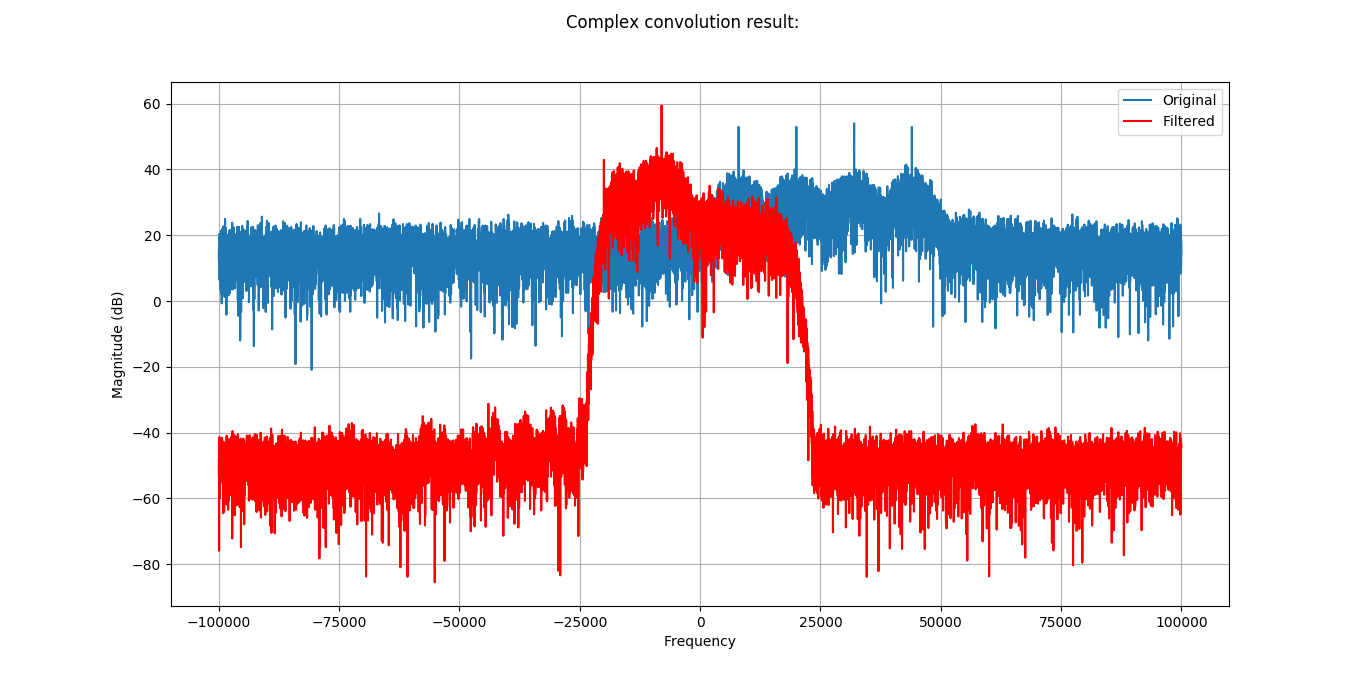
\includegraphics[width=\textwidth]{pics/result.png}
           \captionsetup{justification=centering}
           \captionof{figure}{Результат комплексной целочисленной фильтрации 4FSK сигнала. Команда для отображения: {\tt python3 ../scripts/plot\_complex\_int.py}}
       \end{figure}
    \end{frame}
    \begin{frame}
        \begin{center}
        \baselineskip 20.0mm
        \Huge Спасибо за внимание!
        \end{center}
    \end{frame}
\end{document}